% Optimizer comparison report for GEKO coefficient calibration.
%
% Written as a standalone, appendix-style document (top-level headings are
% \section, not \chapter) so it can be compiled on its own (e.g. via Overleaf --
% no local LaTeX distribution is available in this environment) or have its
% body \input{} into an existing report's appendix.  If embedding, demote every
% \section -> \subsection (or add \addtocounter{section}{...} as needed) and
% drop the preamble down to \begin{document}.
%
% Figures are read from optimizer_visualization/plots/comparison/{1d,2d}/ --
% compile from within optimizer_visualization/, or adjust \graphicspath.

\documentclass[11pt]{article}

\usepackage[margin=1in]{geometry}
\usepackage{graphicx}
\usepackage{booktabs}
\usepackage{amsmath}
\usepackage{hyperref}
\hypersetup{colorlinks=true, linkcolor=blue, citecolor=blue, urlcolor=blue}

\graphicspath{{plots/comparison/1d/}{plots/comparison/2d/}}

\newcommand{\csep}{C_{sep}}
\newcommand{\cnw}{C_{nw}}

\title{Optimizer Comparison for GEKO Coefficient Calibration\\[2pt]
\large Periodic Hills, $Re_h = 2800$}
\author{}
\date{}

\begin{document}
\maketitle

\section{Purpose and Scope}

This appendix documents a benchmark comparing seven optimization strategies for
calibrating GEKO turbulence-model coefficients against DNS reference data, run on
the periodic hills test case at $Re_h = 2800$. Its purpose is to justify the choice
of Bayesian Optimization (BO) as the project's primary optimizer, and to show that
Particle Swarm Optimization (PSO) is a viable, trivially parallelizable alternative
(Section~\ref{sec:pso}).

All seven strategies were run twice: once tuning a single coefficient ($\csep$,
Section~\ref{sec:results-1d}) and once tuning two coefficients jointly ($\csep$ and
$\cnw$, Section~\ref{sec:results-2d}). Every run shares the same fixed simulation
setup and cost function (Section~\ref{sec:costfn}); only the proposed coefficient
values change between evaluations. Before being applied to the real CFD case, the
same optimizer implementations were first validated on cheap analytic test
functions designed to expose specific failure modes (local-minimum traps,
non-smooth landscapes); those synthetic benchmarks are not repeated here. A
further extension of this study, jointly tuning five GEKO coefficients, is
planned and will be added to Section~\ref{sec:results-5d} once available.

\section{Test Case and Cost Function}
\label{sec:costfn}

\subsection{Fixed simulation setup}

Every evaluation, regardless of optimizer, solves the same RANS case in Ansys
Fluent:

\begin{itemize}
  \item \textbf{Geometry:} periodic hills, hill height $H=1$ (normalized),
        spanwise-to-hill-height ratio $l_y/H = 3.035$, fixed mesh (structured
        quad cells, $7.2$--$21.6\,\mathrm{mm}$ cell size, $22$ near-wall
        inflation layers, first layer height $0.72\,\mathrm{mm}$, growth rate
        $1.15$--$1.2$).
  \item \textbf{Flow:} $Re_h = 2800$ (fluid density $1.0$, viscosity
        $3.5714\times10^{-4}$), $200$ solver iterations per evaluation, residual
        convergence targets of $10^{-5}$ on continuity, both velocity
        components, $k$, and $\omega$.
  \item \textbf{DNS reference:} time-averaged periodic-hills DNS field data at
        $Re_h=2800$ on the standard Breuer/Mellen/Fr\"ohlich hill geometry
        \cite{breuer2009}, pre-processed into a fixed columnwise ASCII file.
\end{itemize}

Only the geometry, mesh, solver settings, and DNS reference are held fixed across
\emph{every} evaluation of \emph{every} optimizer in this study --- the only thing
that varies between evaluations is the proposed GEKO coefficient vector
$\mathbf{c}$.

\subsection{Free parameters}

\begin{center}
\begin{tabular}{@{}lccc@{}}
\toprule
Coefficient & Study & Bounds & GEKO default \\
\midrule
$\csep$ & 1D and 2D & $[0.7,\ 2.5]$ & $1.75$ \\
$\cnw$   & 2D only   & $[-2.0,\ 2.0]$ & $0.5$ \\
\bottomrule
\end{tabular}
\end{center}

The 1D study holds $\cnw$ fixed at its GEKO default; the 2D study tunes both
coefficients jointly.

\subsection{The GEDCP cost function}

The optimizer minimizes a single scalar score, the \emph{General Error and
Default-Coefficient Preference} (GEDCP) score. It combines a field-matching error
against DNS with a mild penalty for straying from GEKO's own recommended
defaults:

\begin{equation}
f(\mathbf{c}) \;=\; E_F(\mathbf{c}) \cdot \Bigl(1 + \lambda_p\, p(\mathbf{c})\Bigr),
\qquad \lambda_p = 0.5
\label{eq:gedcp}
\end{equation}

\paragraph{Field error $E_F$.} An \emph{unweighted} sum, over five DNS-observed
fields $\Phi = \{U_x,\, U_y,\, k,\, P_k,\, \varepsilon\}$ (streamwise velocity,
wall-normal velocity, turbulent kinetic energy, production of $k$, and
turbulent dissipation rate), of the spatially area-weighted,
DNS-standard-deviation-normalized $L_2$ error between simulation and DNS:

\begin{equation}
E_F(\mathbf{c}) \;=\; \sum_{\phi \in \Phi}
\sqrt{\; \dfrac{\displaystyle\sum_{i} w_i \left(\dfrac{\phi^{DNS}_i - \phi^{sim}_i(\mathbf{c})}{\sigma^{DNS}_\phi}\right)^{\!2}}
{\displaystyle\sum_i w_i} \;}
\label{eq:fielderr}
\end{equation}

where $i$ indexes DNS sample points and $w_i$ is each point's cell-area weight
(so a densely sampled region does not dominate the score merely by node
count) -- this is a \emph{spatial} weighting within a single field's error,
not a weighting between fields. $\sigma^{DNS}_\phi$ is the area-weighted
standard deviation of DNS field $\phi$, which rescales each field's residual
into units of that field's own natural variability so the five terms are on
comparable scales; every field is then summed with equal weight ($=1$), not a
tuned or field-specific coefficient -- the implementation used here hardcodes
this equal weighting and does not expose a way to change it per field.
DNS points that fall inside (or on) the analytic hill surface are excluded
from every statistic above, so the comparison covers only the shared fluid
region. The simulation field is interpolated onto the (masked) DNS points
before the error is taken.

\paragraph{Coefficient preference $p$.} A mean relative deviation of the
optimized coefficients from their GEKO defaults:

\begin{equation}
p(\mathbf{c}) \;=\; \frac{1}{|\mathbf{c}|} \sum_{j} \left| \frac{c_j^{default} - c_j}{c_j^{default}} \right|
\label{eq:pref}
\end{equation}

summed only over the coefficient(s) actually being tuned in a given study (i.e.\
just $\csep$ in the 1D study; $\csep$ and $\cnw$ in the 2D study). This term
gently discourages the optimizer from finding a numerically better but physically
implausible coefficient combination far from GEKO's recommended operating range.

Both the pure integral-quantity error term ($E_I$) and its weight are disabled
($\lambda_I = 0$) for every configuration in this study, so Eq.~\eqref{eq:gedcp}
reduces to $f(\mathbf{c}) = E_F(\mathbf{c})\,(1 + 0.5\,p(\mathbf{c}))$ in practice.
As a reference point, the GEKO-default simulation ($\csep=1.75$, $\cnw=0.5$,
$p=0$) scores $f = 2.9781$ under this metric in both studies.

\section{Optimization Strategies Compared}
\label{sec:strategies}

Seven strategies were compared, each given the same total evaluation budget: $21$
evaluations in the 1D study, $60$ in the 2D study.\footnote{\texttt{BO\_2D\_ph2800}'s
recorded run used 70 evaluations rather than 60.}

\subsection{Bayesian Optimization (BO)}

A Gaussian-process surrogate (\texttt{skopt}, Mat\'ern kernel with $\nu=2.5$, $10$
restarts of the kernel hyperparameter fit) over Expected Improvement. The run
starts with a batch of Sobol quasi-random samples before switching to
model-guided proposals:

\begin{center}
\begin{tabular}{@{}lccc@{}}
\toprule
Study & Total evals & Sobol samples & Model-guided evals \\
\midrule
1D & 21 & 7  & 14 \\
2D & 60 & 13 & 47 \\
\bottomrule
\end{tabular}
\end{center}

These kernel and estimator settings were not tuned for this case; they were
adopted directly from \cite{bo_hyperparams_ref}. See
Section~\ref{sec:future-work} for the corresponding gap in the other
optimizers.

\subsection{Nelder--Mead (NM)}

A derivative-free simplex method, initialized on a startup simplex centered on
the GEKO defaults ($\pm 0.1$ offset per dimension). Reflection/expansion/
contraction/shrink coefficients: $\alpha=0.8$, $\gamma=1.5$, $\rho=0.5$,
$\sigma=0.5$ (a less aggressive reflection and expansion than the textbook
defaults of $1.0$/$2.0$, chosen since the CFD cost surface near the optimum
behaves like a smooth bowl where overshoot is more costly than slow reflection).

\subsection{Finite Differences (FD)}

Classic forward-difference gradient descent. Each cycle: probe every dimension
once ($\text{base} + \delta_i \, e_i$), estimate the gradient, then take one
descent step $\text{base} - \eta\,\nabla f$. The step is accepted
\emph{unconditionally} as the new base for the next cycle -- there is no
``keep-best'' check, so \texttt{best-so-far} (not last-iterate) is what is
reported in Section~\ref{sec:results}. The probe perturbation
$\delta_i = \text{clip}\bigl((\text{high}_i-\text{low}_i)\cdot\text{step\_size},\ \text{min\_step},\ \text{max\_step}\bigr)$,
with $\text{min\_step}=10^{-5}$, $\text{max\_step}=0.25$ in every configuration
below.

\begin{center}
\begin{tabular}{@{}llcc@{}}
\toprule
Config & Role & step\_size & learning\_rate $\eta$ \\
\midrule
1D standalone FD & exploration from scratch & $0.05$ & $0.2$ \\
1D BO$\to$FD     & exploitation, tightened   & $0.03$ & $0.1$ \\
2D standalone FD & exploration from scratch & $0.05$ & $0.075$ \\
2D BO$\to$FD     & exploitation, tightened   & $0.03$ & $0.045$ \\
\bottomrule
\end{tabular}
\end{center}

\subsection{Hybrid strategies}

Two hybridization patterns were tested, each combining BO with a heuristic
method (NM or FD) in a different order:

\paragraph{Warm-start: FD$\to$BO and NM$\to$BO.} The heuristic method runs
\emph{first}, with no prior knowledge of the optimum, then hands its evaluation
history to BO as a warm start (BO's own model-based search continues from
there instead of from scratch). The heuristic phase uses the exact same NM/FD
parameters as the standalone runs above.

\paragraph{Refinement: BO$\to$NM and BO$\to$FD.} BO explores \emph{first} and
maps out the landscape; its best point is then handed to NM or FD as a starting
point for local refinement. Because BO has already localized a promising region,
the refinement phase is deliberately tightened relative to the standalone
settings to prioritize exploitation over exploration:
\begin{itemize}
  \item \textbf{BO$\to$NM:} the NM startup simplex is rebuilt around BO's best
        point, scaled to $60\%$ of its normal size (\texttt{simplex\_scale=0.6}).
  \item \textbf{BO$\to$FD:} \emph{this is the case worth calling out explicitly}
        -- the FD phase uses a smaller \texttt{step\_size} and
        \texttt{learning\_rate} than standalone FD for its final iterations
        ($0.03$ vs.\ $0.05$ for step\_size; roughly half the learning rate, see
        the table above), so the gradient estimate is more local and the
        descent step does not overshoot the region BO already identified as
        promising. The BO best point is injected directly as the FD starting
        base \emph{without} re-evaluating it, so the first FD iteration begins
        probing immediately.
\end{itemize}

\begin{center}
\begin{tabular}{@{}lccc@{}}
\toprule
& \multicolumn{2}{c}{1D (21 evals)} & 2D (60 evals) \\
Strategy & Phase 1 & Phase 2 & Phase 1 / Phase 2 \\
\midrule
FD $\to$ BO  & FD: 7           & BO: 14 & FD: 13 / BO: 47 \\
NM $\to$ BO  & NM: 7           & BO: 14 & NM: 13 / BO: 47 \\
BO $\to$ NM  & BO: 14 (7 Sobol + 7 GP) & NM: 7 & BO: 23 (13 Sobol + 10 GP) / NM: 37 \\
BO $\to$ FD  & BO: 14 (7 Sobol + 7 GP) & FD: 7 & BO: 23 (13 Sobol + 10 GP) / FD: 37 \\
\bottomrule
\end{tabular}
\end{center}

\subsection{Boundary handling}

Neither NM nor FD clip proposals to the parameter bounds: a simplex reflection or
a gradient step is evaluated exactly where proposed, even if that lies outside
the nominal range. A poor score there is enough to steer the search back without
any explicit correction. BO itself only ever proposes points inside the bounds by
construction.

\section{Results}
\label{sec:results}

Reported scores are the best (minimum) GEDCP score found over the run, computed
from the actual recorded per-iteration results, not a re-derived or estimated
value. For reference, the GEKO-default configuration scores $f=2.9781$ in both
studies.

\subsection{One-dimensional study ($\csep$ only)}
\label{sec:results-1d}

\begin{center}
\begin{tabular}{@{}lccc@{}}
\toprule
Strategy & Evals & Best score $f$ & Best $\csep$ \\
\midrule
Bayesian Optimization & 21 & 2.4577 & 0.8866 \\
Nelder--Mead          & 21 & 2.4577 & 0.8858 \\
Finite Differences    & 21 & 2.4586 & 0.8896 \\
FD $\to$ BO           & 21 & 2.4577 & 0.8877 \\
NM $\to$ BO           & 21 & 2.4577 & 0.8861 \\
BO $\to$ NM           & 21 & 2.4577 & 0.8874 \\
BO $\to$ FD           & 21 & 2.4577 & 0.8874 \\
\midrule
GEKO default (baseline) & -- & 2.9781 & 1.75 \\
\bottomrule
\end{tabular}
\end{center}

All seven strategies converge to essentially the same score ($f \approx 2.4577$,
$\csep \approx 0.886$--$0.890$) -- an $\approx 17\%$ reduction from the GEKO
default. Unlike the deliberately bimodal synthetic benchmark function, the real
1D CFD cost surface behaves close to unimodal over the tested range: no strategy
gets trapped away from the others' optimum. Standalone FD is the only outlier,
settling $\approx 0.04\%$ higher than the rest -- consistent with its
unconditional-accept step (Section~\ref{sec:strategies}), which can wander past
the minimum after finding it.

\begin{center}
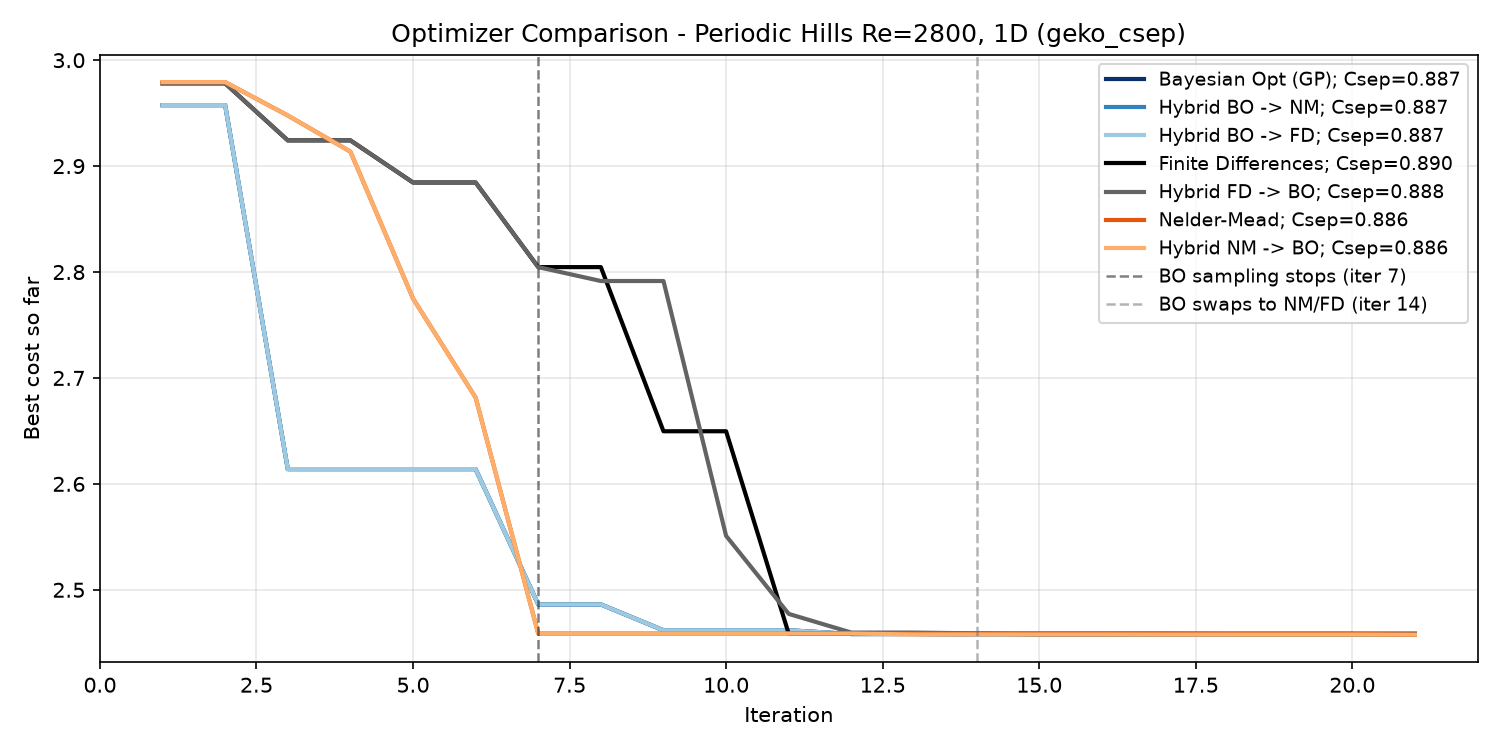
\includegraphics[width=\textwidth]{optimizer_comparison_1d_full.png}
\end{center}
\begin{center}
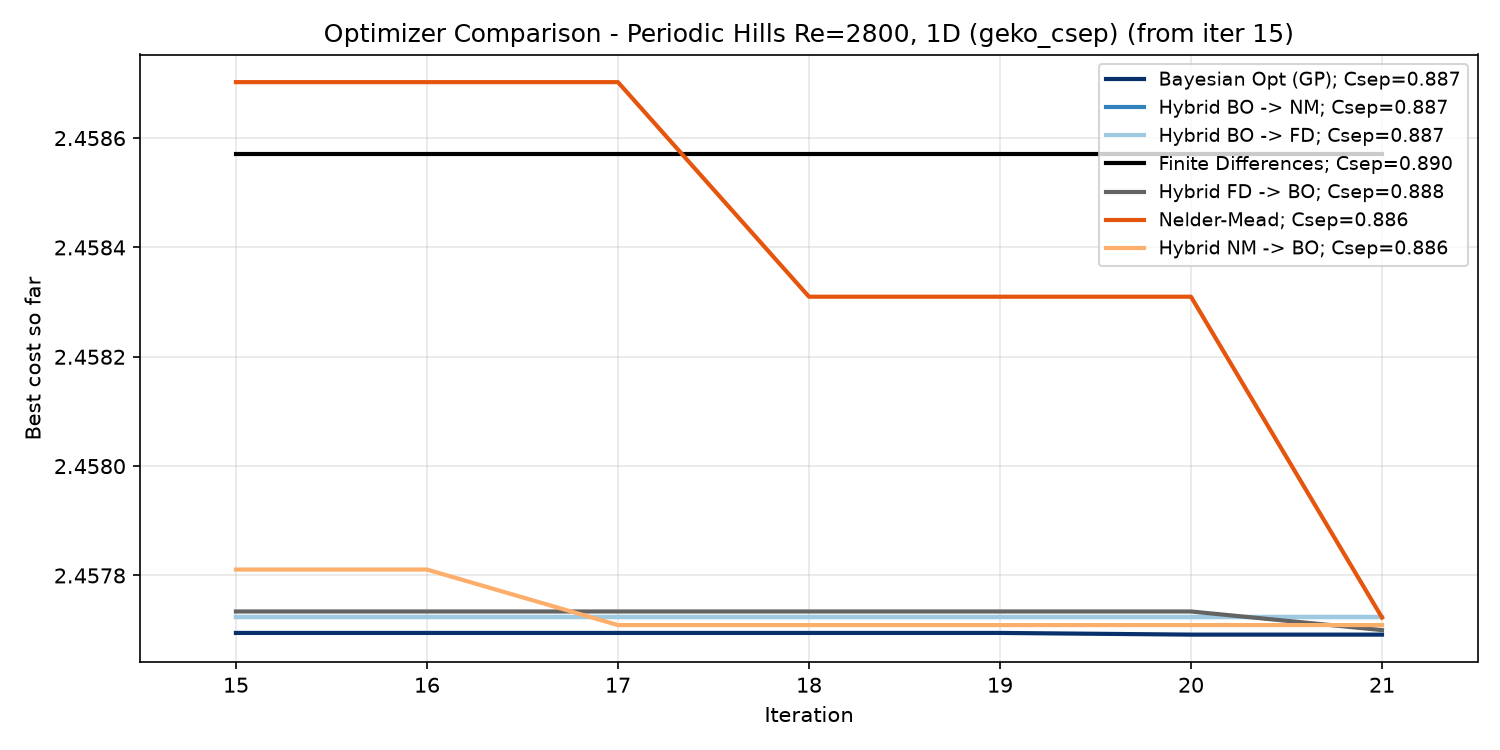
\includegraphics[width=\textwidth]{optimizer_comparison_1d_after_iter14.png}
\end{center}

\subsection{Two-dimensional study ($\csep$, $\cnw$)}
\label{sec:results-2d}

\begin{center}
\begin{tabular}{@{}lcccc@{}}
\toprule
Strategy & Evals & Best score $f$ & Best $\csep$ & Best $\cnw$ \\
\midrule
Bayesian Optimization & 70 & 2.2144 & 0.8730 & 0.4996 \\
Nelder--Mead          & 60          & 2.2135 & 0.8763 & 0.5000 \\
Finite Differences    & 60          & 2.3164 & 0.8360 & 0.4120 \\
FD $\to$ BO           & 60          & 2.2154 & 0.8722 & 0.4988 \\
NM $\to$ BO           & 60          & 2.2212 & 0.8715 & 0.4927 \\
BO $\to$ NM           & 60          & 2.2135 & 0.8764 & 0.4999 \\
BO $\to$ FD           & 60          & 2.2284 & 0.8854 & 0.5145 \\
\midrule
GEKO default (baseline) & -- & 2.9781 & 1.75 & 0.5 \\
\bottomrule
\end{tabular}
\end{center}

\begin{center}
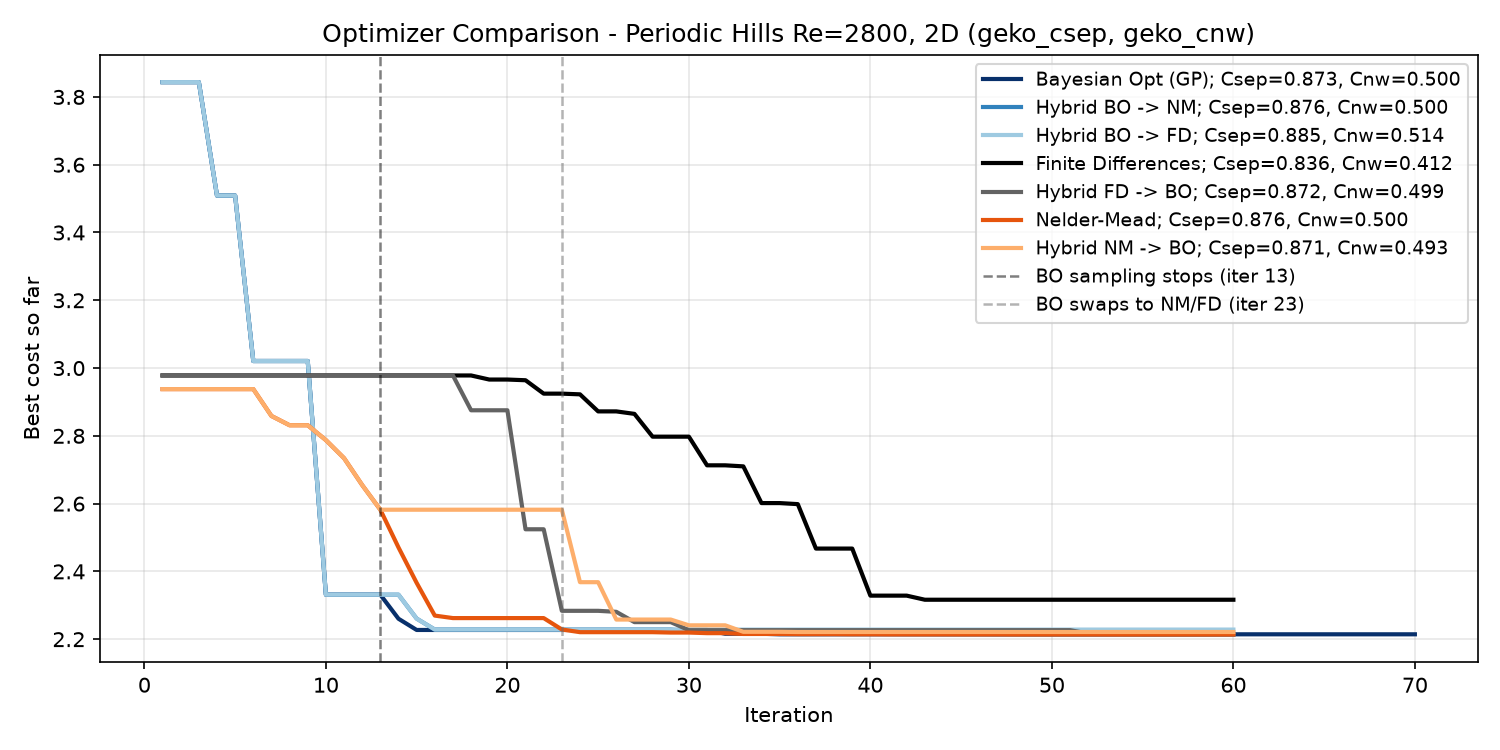
\includegraphics[width=\textwidth]{optimizer_comparison_2d_full.png}
\end{center}
\begin{center}
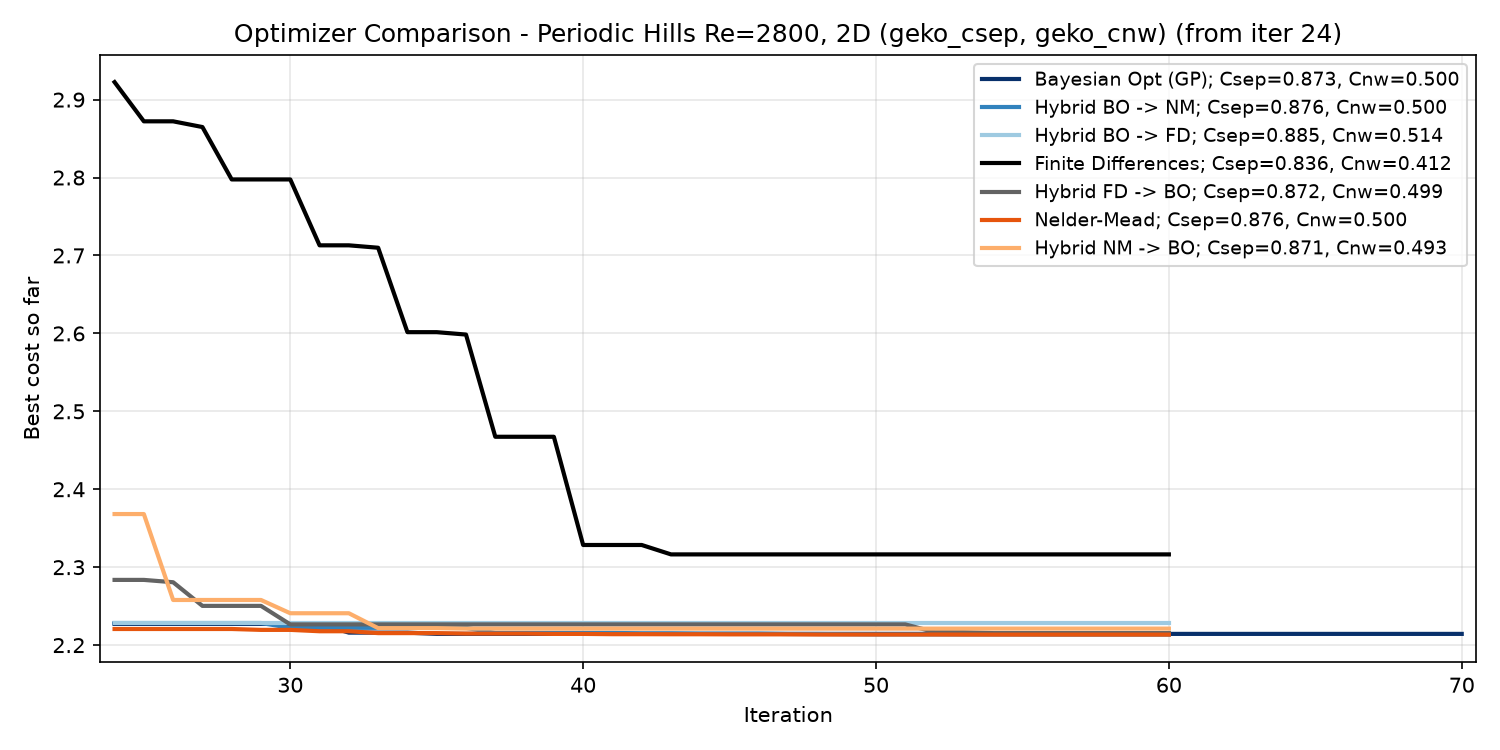
\includegraphics[width=\textwidth]{optimizer_comparison_2d_after_iter23.png}
\end{center}

The 2D study tells a different story than the 1D study: BO, NM, and their
warm-started hybrid (FD$\to$BO) all reach $f \approx 2.213$--$2.215$, essentially
tied. Strategies that lean on FD's gradient estimate in two dimensions do
comparatively worse: BO$\to$FD reaches only $f=2.228$, and standalone FD is
worst overall at $f=2.316$. Adding $\cnw$ as a
free dimension does improve on the 1D-only result ($2.213$--$2.215$ vs.\ $2.458$),
but the best-found $\cnw \approx 0.49$--$0.50$ across every strategy sits almost
exactly on its GEKO default of $0.5$ -- most of the joint-tuning benefit is
concentrated in $\csep$, not $\cnw$.

\subsection{Does the refinement phase actually help?}
\label{sec:refinement-effectiveness}

The BO$\to$NM and BO$\to$FD hybrids are designed so that a cheap
local-refinement phase improves on whatever BO already found. Whether that
happened in practice can be checked directly, by asking which iteration
produced each run's reported best score, and whether that iteration fell
before or after the phase boundary:

\begin{center}
\begin{tabular}{@{}lcccl@{}}
\toprule
Strategy & Study & Phase boundary & Best found at iter. & Refinement improved on BO? \\
\midrule
BO $\to$ NM & 1D & 14 & 14 & No -- best is BO's own last point \\
BO $\to$ FD & 1D & 14 & 14 & No -- best is BO's own last point \\
BO $\to$ NM & 2D & 23 & 59 & Yes -- improved through iter.\ 59/60 \\
BO $\to$ FD & 2D & 23 & 16 & No -- best found inside the BO phase itself \\
\bottomrule
\end{tabular}
\end{center}

In three of the four cases tested, the refinement phase contributed no
improvement at all over what BO had already found by the time it handed off:
in both 1D hybrids the reported best is exactly BO's last evaluation before the
swap, and in 2D, BO$\to$FD's best point was found at iteration 16, seven
iterations \emph{before} the BO phase even ended at iteration 23 -- meaning
neither the remainder of the BO phase nor any of the following 37 FD
evaluations improved on it. The one exception, BO$\to$NM in 2D, kept improving
through the very last swarm iteration, showing the refinement idea can work but
did not reliably do so here. With only one run per configuration
(Section~\ref{sec:strategies}), this is not evidence that refinement is
useless in general -- but on this evidence, BO$\to$FD's tightened step size and
learning rate (Section~\ref{sec:strategies}) never got a chance to demonstrate
an advantage, since FD was never handed a starting point better than the one BO
had already found on its own.

\section{Extended Study: Five-Dimensional Coefficient Calibration}
\label{sec:results-5d}

\textit{Pending -- a further optimizer-comparison run, jointly tuning five GEKO
coefficients against the current objective, is planned but not yet complete.
This section will report its methodology and results once available.}

\section{Discussion}

Taken together, these results support Bayesian Optimization as the default
choice for GEKO coefficient calibration on this class of problem:

\begin{itemize}
  \item \textbf{No hand-tuned step size.} FD requires a learning rate calibrated
        to the (unknown, and possibly direction-dependent) local curvature of
        the cost surface; getting it wrong is not just a matter of slower
        convergence -- it visibly cost FD accuracy in the 2D study. BO makes no
        such assumption.
  \item \textbf{Comparable or better minima in the harder (2D) case.} BO, NM,
        and BO's own hybrids match or beat every FD-involving strategy in the
        2D study, while all methods are statistically indistinguishable in the
        easier 1D study. The real advantage of a global surrogate model shows
        up precisely as the problem gets harder, which is the direction this
        project's future work (more coefficients, more cases) is headed.
  \item \textbf{Principled warm-starting.} The hybrid strategies show that BO
        can productively consume another optimizer's history (FD$\to$BO,
        NM$\to$BO) or hand off to one for cheap local refinement (BO$\to$NM,
        BO$\to$FD) without ever losing accuracy, giving flexibility that a
        standalone heuristic method does not offer on its own -- though as
        Section~\ref{sec:refinement-effectiveness} shows, the refinement phase
        does not always add measurable value beyond BO's own result: it did in
        2D for BO$\to$NM, but not for BO$\to$FD in either dimension tested.
\end{itemize}

The synthetic benchmark's local-vs-global trap is not strongly visible in this
specific real-CFD range -- the 1D cost surface tested here is closer to unimodal
than the adversarial analytic test function. That does not undercut the case for
BO: the GEKO parameter space explored elsewhere in this project (more
coefficients, wider bounds) is exactly where a smoother, better-behaved region
like this one is the exception rather than the rule, and BO's
exploration/exploitation balance costs nothing when the landscape happens to be
easy.

\section{Particle Swarm Optimization}
\label{sec:pso}

Alongside the seven strategies above, a particle-count sweep of Particle Swarm
Optimization (PSO) was run in both dimensions, to check whether it reaches
comparable optima to BO/NM while being structurally parallelizable across
concurrent Fluent sessions (its particles are, by construction, independent
within a swarm iteration), unlike the inherently sequential ask/tell loop of
BO, NM, and FD. Every run in this sweep was still executed sequentially, one
particle at a time; actually exploiting this parallelism has not yet been
implemented (see Section~\ref{sec:future-work}).

\subsection{Configuration}
\label{sec:pso-config}

Each particle moves under the standard velocity update
$v \leftarrow w v + c_1 r_1 (\mathbf{x}_{pbest}-\mathbf{x}) + c_2 r_2 (\mathbf{x}_{gbest}-\mathbf{x})$,
with $r_1, r_2 \sim \mathcal{U}(0,1)$ drawn independently per particle and per
dimension, and inertia $w$ decaying linearly from $w_{start}$ to $w_{end}$ over
the swarm iterations. Velocity is clamped component-wise to
$\pm v_{max}$ (a fixed fraction of that dimension's range); a particle that
would overshoot a bound is pinned exactly to it and that velocity component is
zeroed (boundary absorption -- the one optimizer in this study that \emph{does}
clip). Initial particle positions are drawn from a Sobol sequence, the same
quasi-random mechanism used for BO's initial sampling, rather than uniform
random placement.

The following hyperparameters are identical across every PSO run in this
study, in both dimensions:

\begin{center}
\begin{tabular}{@{}cccccc@{}}
\toprule
$w_{start}$ & $w_{end}$ & $c_1$ & $c_2$ & $v_{max}$ & random\_state \\
\midrule
$0.9$ & $0.2$ & $1.5$ & $1.5$ & $0.1 \times$ range & $1$ \\
\bottomrule
\end{tabular}
\end{center}

Only the particle count and the total evaluation budget change across the
sweep. The number of swarm iterations is derived, not configured directly:
$\text{iterations} = \lfloor \text{evals} / \text{particles} \rfloor - 1$
(the initial Sobol sweep costs one evaluation per particle, and each
subsequent swarm iteration costs one evaluation per particle again). Because
the evaluation budget
for each sweep point is chosen as the multiple of its particle count closest to
a common target ($\approx 40$ evaluations in 1D, $\approx 75$--$80$ in 2D, so
that runs with different particle counts remain roughly comparable in total
cost), more particles mechanically means fewer swarm iterations:

\begin{center}
\begin{tabular}{@{}lccc@{}}
\toprule
Study & Particles & Evals & Swarm iterations \\
\midrule
1D & 3  & 39 & 12 \\
1D & 5  & 40 & 7  \\
1D & 7  & 42 & 5  \\
1D & 9  & 36 & 3  \\
2D & 10 & 80 & 7  \\
2D & 15 & 75 & 4  \\
2D & 20 & 80 & 3  \\
\bottomrule
\end{tabular}
\end{center}

\subsection{One-dimensional sweep}

\begin{center}
\begin{tabular}{@{}lccc@{}}
\toprule
Particles & Evals & Best score $f$ & Best $\csep$ \\
\midrule
3 & 39 & 2.4577 & 0.8874 \\
5 & 40 & 2.4577 & 0.8853 \\
7 & 42 & 2.4589 & 0.8937 \\
9 & 36 & 2.4620 & 0.9062 \\
\bottomrule
\end{tabular}
\end{center}

\begin{center}
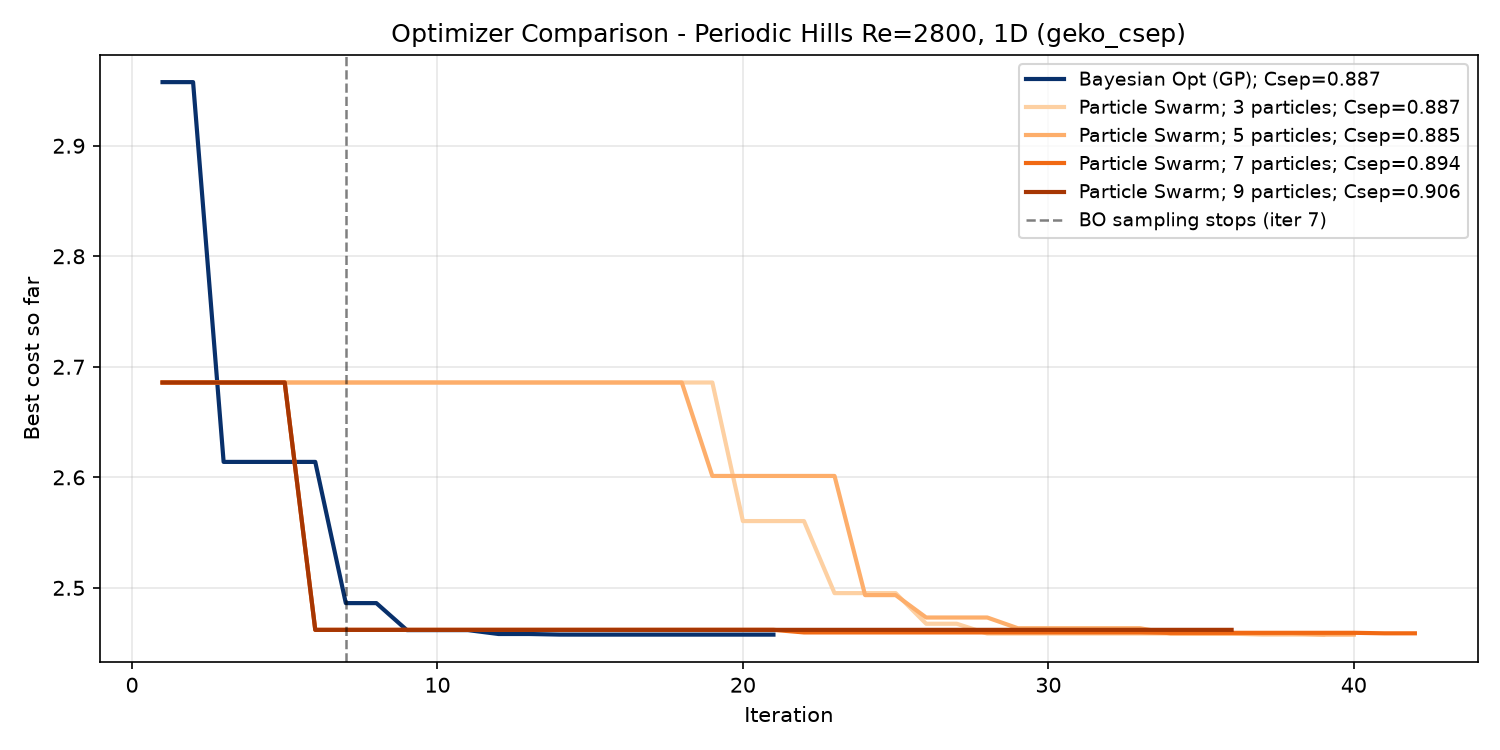
\includegraphics[width=\textwidth]{optimizer_comparison_1d_vs_pso_full.png}
\end{center}
\begin{center}
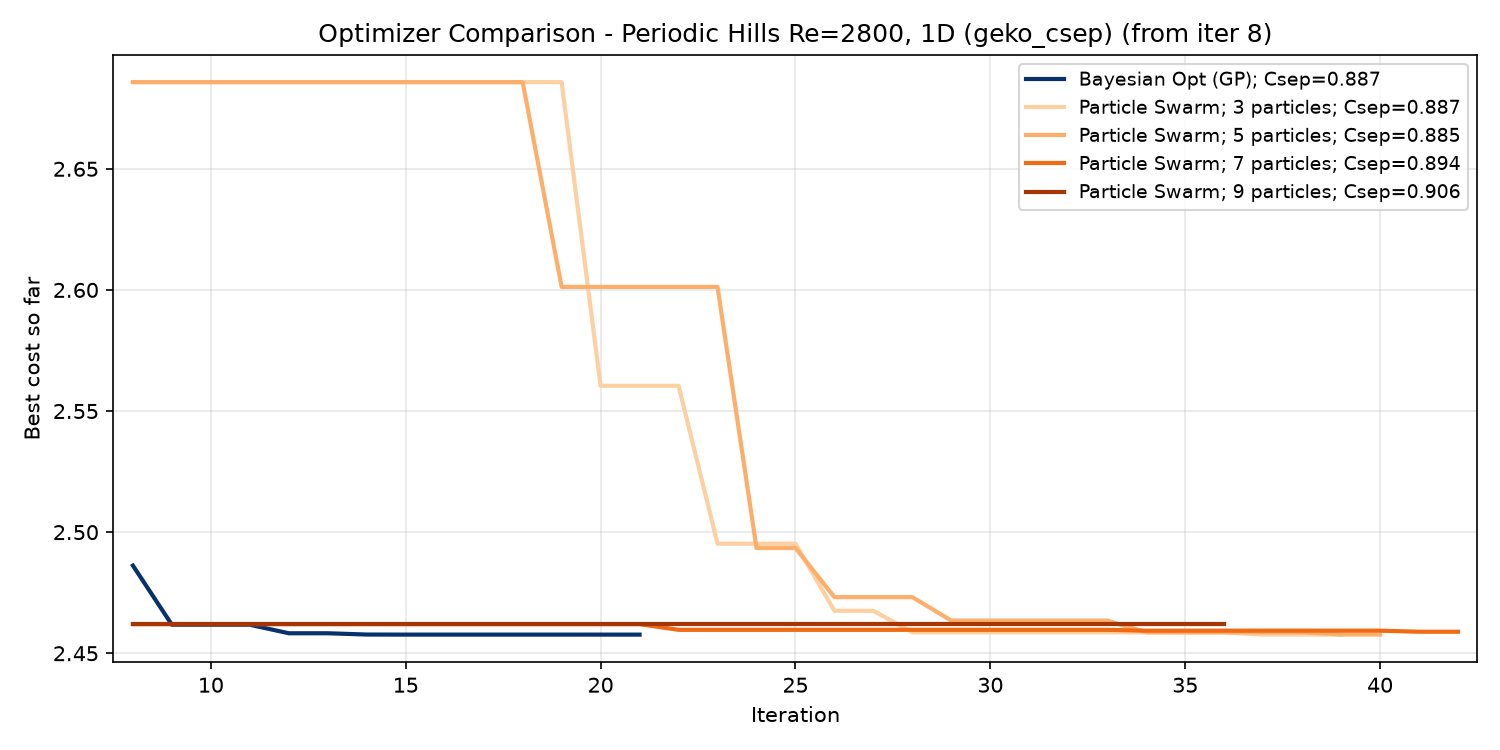
\includegraphics[width=\textwidth]{optimizer_comparison_1d_vs_pso_after_iter7.png}
\end{center}
\begin{center}
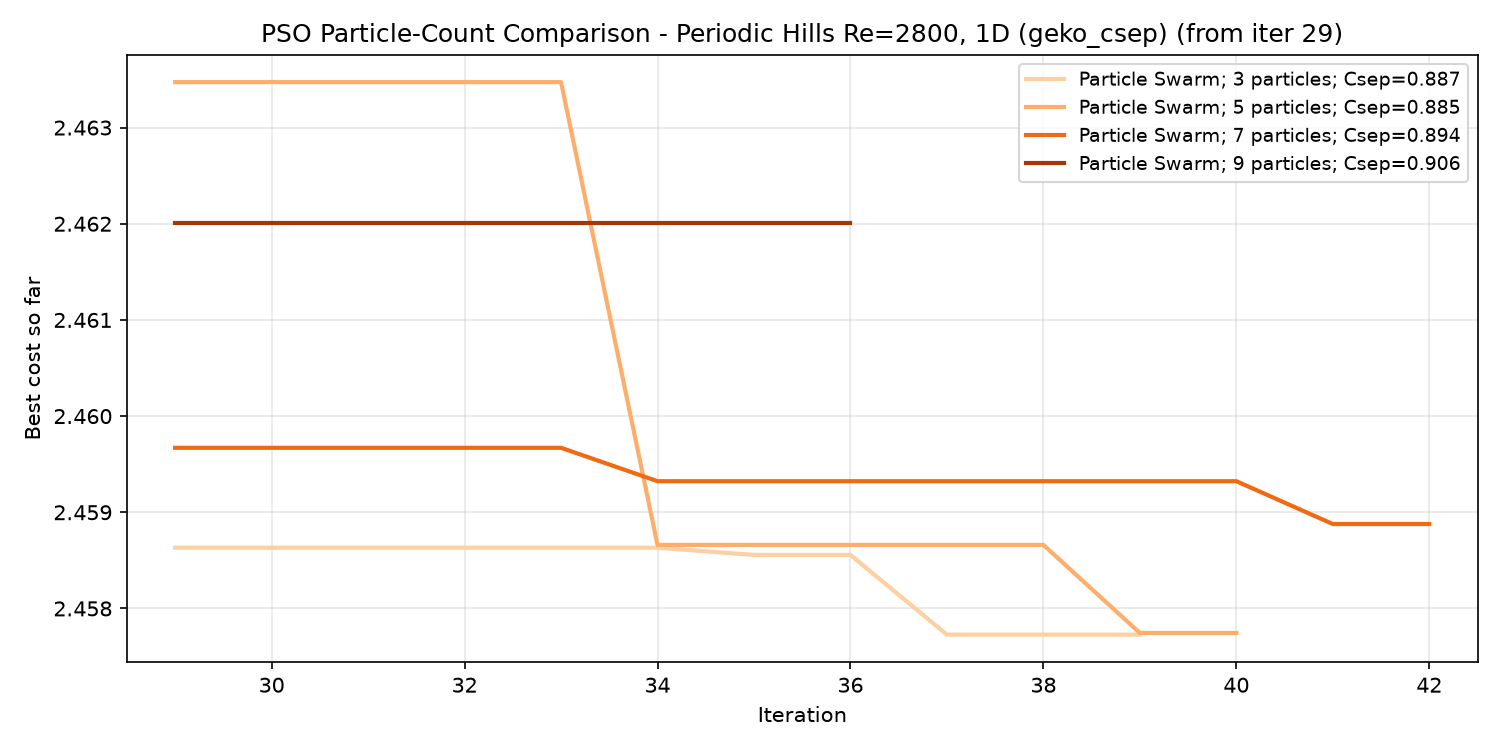
\includegraphics[width=\textwidth]{optimizer_comparison_1d_pso_only_after_iter28.png}
\end{center}

The last figure shows the particle-count sweep alone, without BO: at iteration
28 BO has already exhausted its entire 21-evaluation 1D budget, so it is
dropped from that comparison rather than shown as a flat trailing line.

\subsection{Two-dimensional sweep}

\begin{center}
\begin{tabular}{@{}lccc@{}}
\toprule
Particles & Evals & Best score $f$ & Best $\csep$, $\cnw$ \\
\midrule
10 & 80 & 2.2546 & 0.9442,\ 0.5091 \\
15 & 75 & 2.2285 & 0.8987,\ 0.4909 \\
20 & 80 & 2.2511 & 0.8398,\ 0.4799 \\
\bottomrule
\end{tabular}
\end{center}

\begin{center}
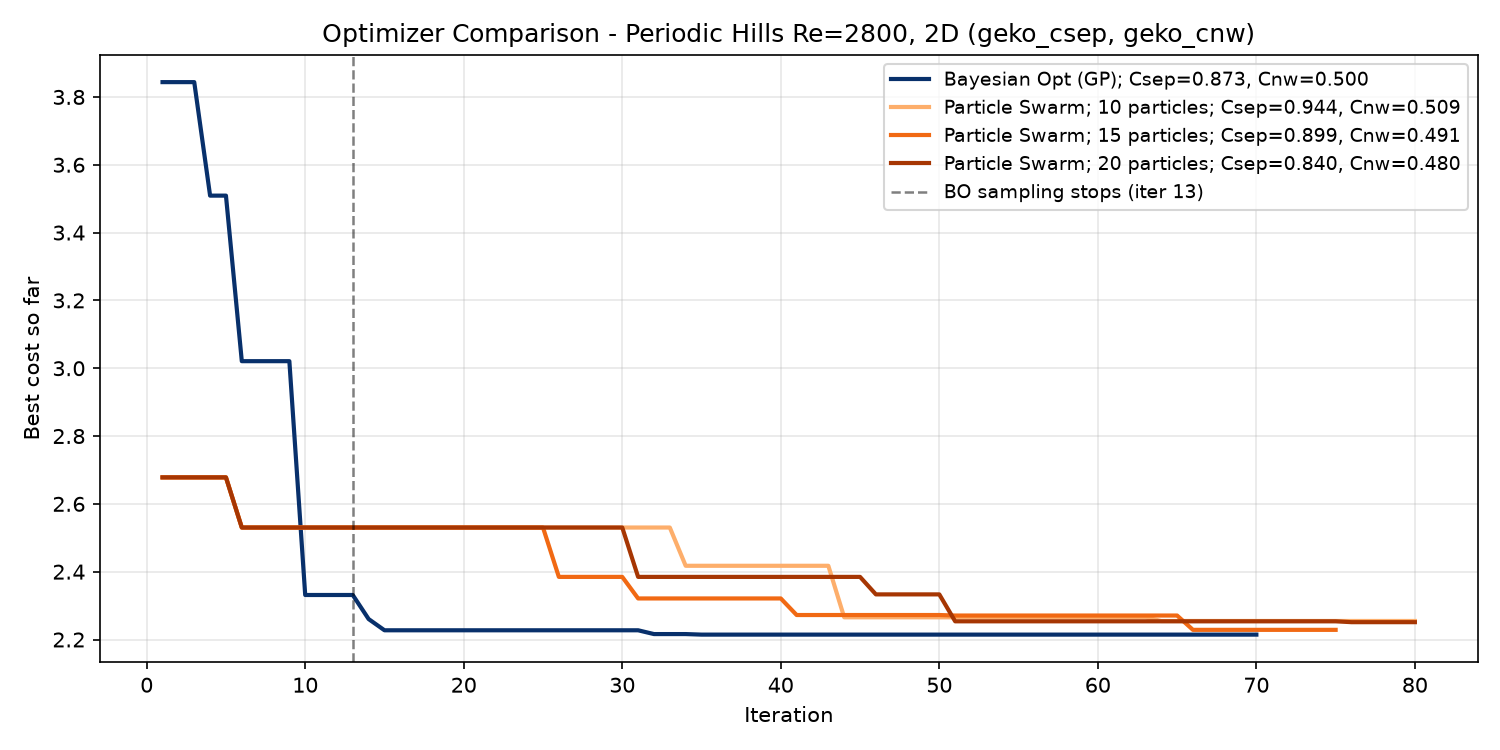
\includegraphics[width=\textwidth]{optimizer_comparison_2d_vs_pso_full.png}
\end{center}
\begin{center}
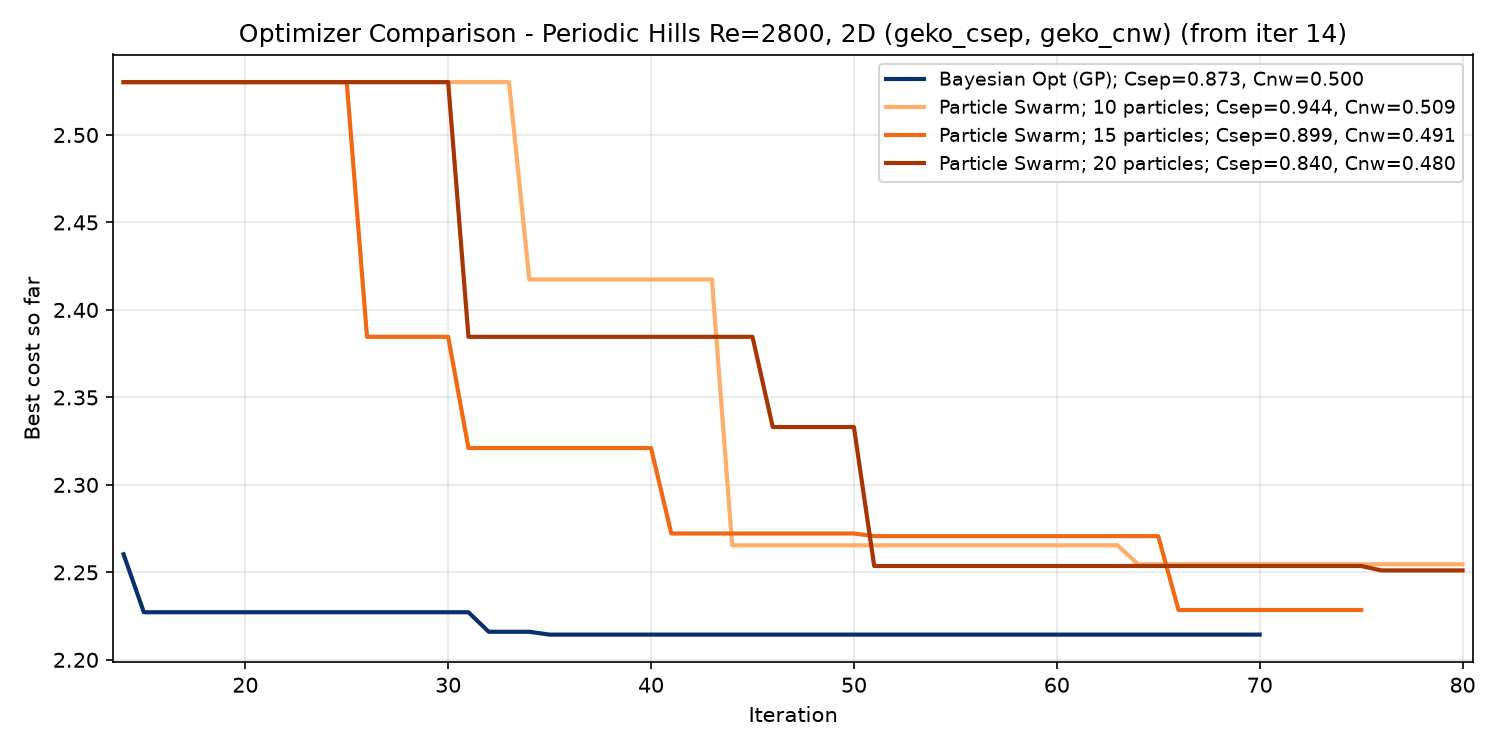
\includegraphics[width=\textwidth]{optimizer_comparison_2d_vs_pso_after_iter13.png}
\end{center}
\begin{center}
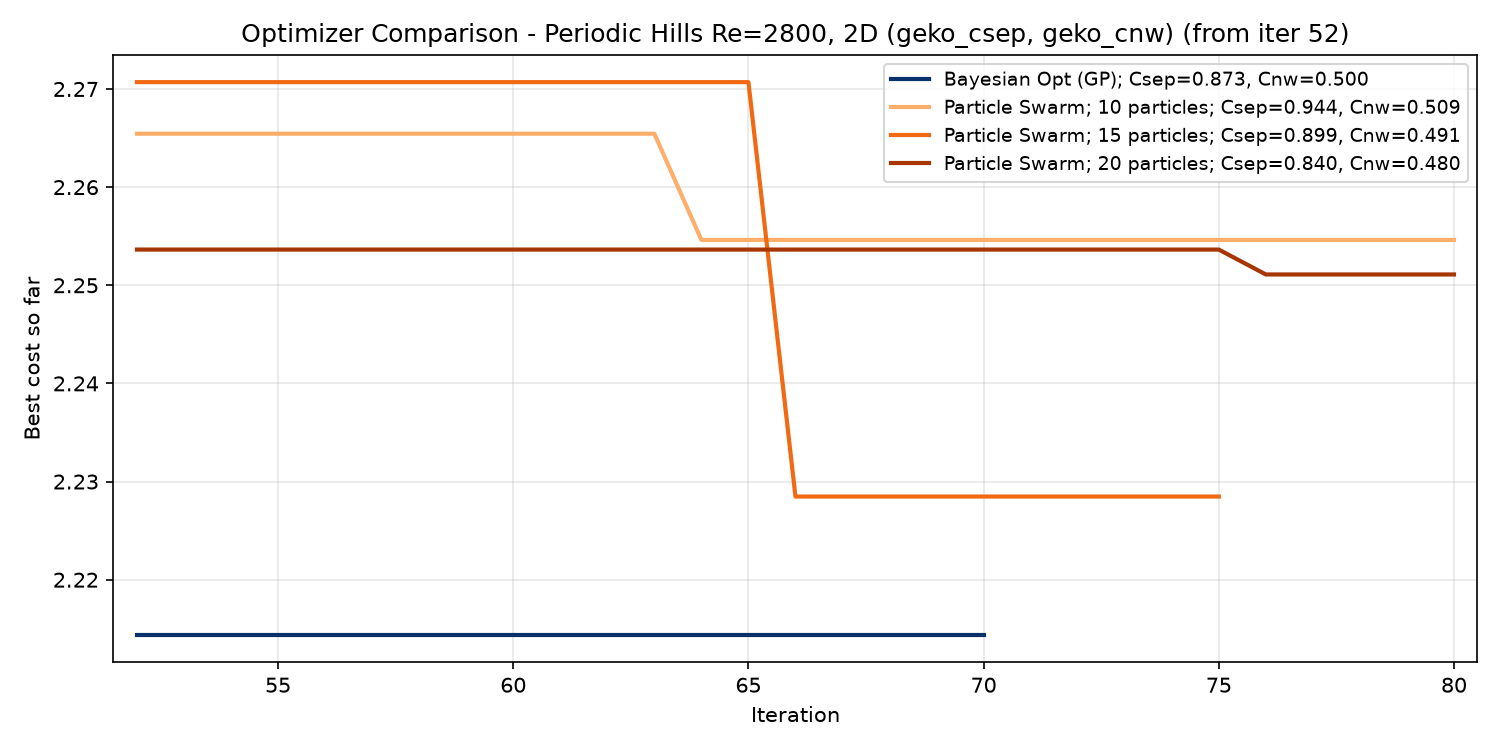
\includegraphics[width=\textwidth]{optimizer_comparison_2d_vs_pso_after_iter51.png}
\end{center}

Here BO's larger recorded budget (70 evaluations, Section~\ref{sec:strategies})
survives even the deepest cutoff, so it remains visible in all three 2D
figures.

\subsection{Discussion}

The 1D sweep degrades monotonically as particle count increases: $f = 2.4577$
(3 particles) $\to 2.4577$ (5) $\to 2.4589$ (7) $\to 2.4620$ (9), tracking the
shrinking swarm-iteration budget in the configuration table above (12
iterations down to 3). With a roughly fixed total evaluation budget, more
particles buys broader coverage per iteration but leaves the swarm far fewer
iterations to actually converge on the optimum it finds -- and in 1D that
trade-off consistently loses. The best two sweep points (3 and 5 particles)
tie BO/NM's 1D optimum exactly at $f=2.4577$.

The 2D sweep does not follow the same clean pattern: 15 particles (4
iterations) beats both 10 particles (7 iterations) and 20 particles (3
iterations), rather than falling neatly between them. Since each particle
count was only run once (consistent with the single-seed scope of this whole
comparison, Section~\ref{sec:strategies}), this is most likely run-to-run
variance rather than a real non-monotonic effect of particle count -- the 1D
sweep's cleaner trend should be trusted more, given it is monotonic across all
four points tested. The best 2D PSO result ($f=2.2285$ at 15 particles) still
trails the BO/NM/BO$\to$NM cluster ($f=2.2135$--$2.2154$, Section~\ref{sec:results-2d})
by about $0.6\%$.

Taken together: PSO ties BO/NM exactly in the easier 1D case and trails by
under $1\%$ in the harder 2D case, across every particle count tried. That is
close enough to make PSO a credible alternative wherever wall-clock time
matters more than the last fraction of a percent of accuracy -- but, as
Section~\ref{sec:future-work} notes, that wall-clock advantage requires
actually running particles concurrently, which this study did not do, and it
presupposes having enough Fluent licenses/compute to match the particle count.
Note also that particle count and swarm-iteration count are confounded in this
sweep by design (Section~\ref{sec:pso-config}): this data cannot
cleanly separate ``more particles helps'' from ``more iterations helps'' as the
driver of the 1D trend.

\section{Limitations and Future Work}
\label{sec:future-work}

\paragraph{Hyperparameter tuning.} With the exception of BO
(Section~\ref{sec:strategies}, whose kernel and estimator settings were adopted
from \cite{bo_hyperparams_ref} rather than tuned for this case), none of the
optimizers' hyperparameters were systematically tuned for the periodic-hills
objective: NM's reflection/expansion/contraction/shrink coefficients and FD's
step size and learning rate were chosen empirically, and PSO's inertia
schedule, cognitive/social coefficients, and velocity cap were carried over
largely unchanged. This was a scope decision driven by time constraints, not a
claim that the values used are optimal. A systematic hyperparameter search --
especially for PSO, whose inertia decay and coefficient choices materially
affect swarm convergence speed -- is left as future work.

\paragraph{PSO parallelization.} Section~\ref{sec:pso} shows PSO reaching
comparable optima to BO/NM, and its particles are, by construction, independent
within a swarm iteration. However, every PSO run in this study was executed
sequentially, one particle at a time, exactly like every other optimizer here.
Actually implementing concurrent particle evaluation (e.g.\ dispatching all
particles in a swarm iteration to separate Fluent sessions at once) has not yet
been done, and is required before PSO's wall-clock advantage can be realized in
practice. See \cite{pso_future_work_ref} for further guidance on parallel PSO
implementation and hyperparameter selection.

\begin{thebibliography}{9}
\bibitem{breuer2009}
M.\ Breuer, N.\ Peller, Ch.\ Rapp, M.\ Manhart,
\emph{Flow over periodic hills -- numerical and experimental study in a wide
range of Reynolds numbers}, Computers \& Fluids, 38(2):433--457, 2009.
% TODO(user): replace this entry with the actual reference for the paper the
% BO kernel/estimator hyperparameters (Matern nu=2.5, 10 kernel restarts,
% Sobol initialization) were adopted from.
\bibitem{bo_hyperparams_ref}
\textit{[reference pending -- to be inserted]}
% TODO(user): replace this entry with the actual reference for the PSO
% parallelization / hyperparameter-tuning paper.
\bibitem{pso_future_work_ref}
\textit{[reference pending -- to be inserted]}
\end{thebibliography}

\end{document}
